\documentclass[10pt]{article}
\usepackage{textcomp}
\usepackage{a4wide}
\usepackage{graphicx}
\usepackage{amsmath}
\usepackage{amsbsy}
\usepackage{amsfonts}
\usepackage{epstopdf, epsfig}
\usepackage{amssymb}
\usepackage{longtable}
\usepackage{mathtools}
\usepackage{textcomp, csquotes}
\usepackage{xfrac} 
\usepackage[inline]{enumitem}
\usepackage{afterpage}
\usepackage{natbib}
\renewcommand{\labelenumi}{(A\arabic{enumi})}
\renewcommand{\theenumi}{(A\arabic{enumi})}
\usepackage{gensymb}
\usepackage{setspace}
\usepackage{geometry}
\geometry{right=.8in,left=.8in,top=1in,bottom=1in}
\usepackage{lineno}
\usepackage[hidelinks,colorlinks=true,linkcolor=blue]{hyperref}
\hypersetup{citecolor=blue, urlcolor=blue}
\usepackage{multirow}
\usepackage{listings}
\usepackage{xcolor}

\definecolor{codegreen}{rgb}{0,0.6,0}
\definecolor{codegray}{rgb}{0.5,0.5,0.5}
\definecolor{codepurple}{rgb}{0.58,0,0.82}
\definecolor{backcolour}{rgb}{0.95,0.95,0.92}

\lstdefinestyle{DOS}
{
    backgroundcolor=\color{black},
    basicstyle=\scriptsize\color{white}\ttfamily
}

\lstdefinestyle{mystyle}{
    backgroundcolor=\color{backcolour},   
    commentstyle=\color{codegreen},
    keywordstyle=\color{magenta},
    numberstyle=\tiny\color{codegray},
    stringstyle=\color{codepurple},
    basicstyle=\ttfamily\footnotesize,
    breakatwhitespace=false,         
    breaklines=true,                 
    captionpos=b,                    
    keepspaces=true,                 
    numbers=left,                    
    numbersep=5pt,                  
    showspaces=false,                
    showstringspaces=false,
    showtabs=false,                  
    tabsize=2
}

\lstset{style=mystyle}

\title{pymm: An open-source image-based framework for CFD in microsystems}
\author{David Landa-Marb\'an}
\date{%
	Energy \& Technology, NORCE Norwegian Research Centre AS, Norway\\
    \today
}

\begin{document}
\pagenumbering{arabic}
\maketitle
\onehalfspace
\vspace{2cm}
\begin{abstract}
\noindent This report describes the adopted approach for the numerical studies on the micromodel system described in \cite{Benali2019,Liu2022}. We used python packages (e.g., porespy \citep{Gostick2019} and skimage \citep{Walt2014}) to generate the spatial domains for the simulations from the microsystem images, and Gmsh \citep{Geuzaine2009} as a mesh generator. The numerical simulations for the water flow and tracer are performed using the OpenFOAM simulator. This framework could be applied to general images and the current implementation could be (``easily") extended to consider further geometry of devices and solvers in OpenFOAM \end{abstract}
\vspace{1.4cm}

\section{Command line options}

The current implementation supports the following argument options:
\begin{lstlisting}[style=DOS]
pymm -i image.png -p parameters.txt -o output -m image -t all -g gmsh
\end{lstlisting}

where
\begin{itemize}
\item -i, -image: The base name of the image (`microsystem.png' by default).
\item -p, -parameters: The base name of the parameter file (`parameters.txt' by default).
\item -m,-mode: The configuration of the microsystem, currently only image and device supported (`image' by default).
\item -t, -type: Run the whole framework (`all'), only the mesh part (`mesh'), keep the current mesh and only the flow (`flow'), flow and tracer (`flowntracer'), or only tracer (`tracer') (`all' by default).
\item -o, -output: The base name of the output folder (`output' by default).
\item -g, -gmsh: The full path to the Gmsh executable or simple `gmsh' if it runs from the terminal (`gmsh' by default).
\end{itemize}

\section{Input image}

Let us consider the image in Fig. \ref{modelo} (this image and the real dimensions can be extracted from Fig. 52 in \cite{Benali2019} and Fig. 1c in \cite{Liu2022}). This image (2D) consists of 805x252 pixels, and the real dimensions (3D) are 6.74e-3 x 2.5e-3 x 0.03e-3 [m]. We remark that the image of the pattern used in the numerical simulations in \cite{Liu2022} has a much higher resolution.
\begin{figure}[h!]
\centering
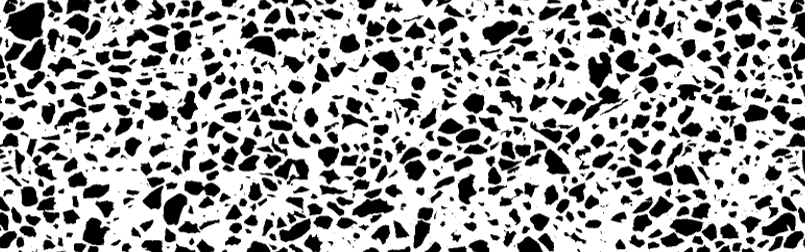
\includegraphics[width=0.7\textwidth]{microsystem.png}
\caption{Grains and pore space configuration.}
\label{modelo} 
\end{figure}

\section{Input parameters}
The current implementation allows for the following input parameters:

\begin{lstlisting}[language=Python]
"""Set the framework parameters"""
6.74e-3     #Image-related, length of the microsystem [m]
2.5e-3      #Image-related, height of the microsystem [m]
0.03e-3     #Image-related, depth of the microsystem [m]
160         #Image-related, threshold for converting the image to binary
1.0         #Image-related, rescaled factor for the input image
100         #Image-related, minimum size of the grain clusters
1.0         #Image-related, tolerance to approximate the border as polygon
1.0         #Image-related, tolerance to approximate the grains as polygon
1.0         #Figure-related, line width to show the contours in the produced figures
0.2e-3      #Device-related, width of the top and bottom channels in the micromodel device [m]
1e-4        #Mesh-related, mesh size [m]
1e-6        #Fluid-related, kinematic viscosity [Dynamic viscosity/fluid_density, m2/s]
1e-12       #Tracer-related, diffusion coefficient [m2/s]
5.0e-4      #Simulation-related, inlet boundary condition (Pressure/fluid_density, [Pa/(kg/m3)])
30.0        #Simulation-related, end time for the tracer simulation [s]
1.0         #Simulation-related, time interval to write the tracer results [s]
1e-7        #Solver-related, convergence criterium for the pressure solution
1e-8        #Solver-related, convergence criterium for the velocity solution
1000        #Solver-related, maximum number of iterations to reach the convergence criteria
1.0         #Solver-related, time step in the numerical scheme for the Tracer simulation [s]
\end{lstlisting}

\subsection{Image-related parameters}
The three first parameters set the real dimensions of the microsystem. The next parameter sets the threshold value to convert the image to binary (valid values from 0 to 255). The rescaled factor parameter reduces the number of pixels of the image (valid values between 0 and 1, see \href{https://scikit-image.org/docs/stable/api/skimage.transform.html#skimage.transform.rescale}{skimage.transform.rescale}). The minimum size of the grain clusters controls the number of pixels to consider for the internal grains (valid values are greater than 0, see \href{https://porespy.org/modules/generated/porespy.filters.trim\_small\_clusters.html}{porespy.filters.trim\_small\_clusters}). The two following parameter, for setting the tolerance to approximate the contours of polygons, reduce the number of points in the extracted border and internal grains respectively (valid values are 0 or greater than 0, see  \href{https://scikit-image.org/docs/stable/auto\_examples/edges/plot\_polygon.html}{skimage.measure.approximate\_polygon}). Figure \ref{sizes} shows the internal grains and border for three decreasing values of the minimum size cluster and tolerances. The smaller are these numbers, the more detail is included in the mesh; however, this increases the execution time to create the mesh and to run the simulations. 

\begin{figure}[h!]
\centering
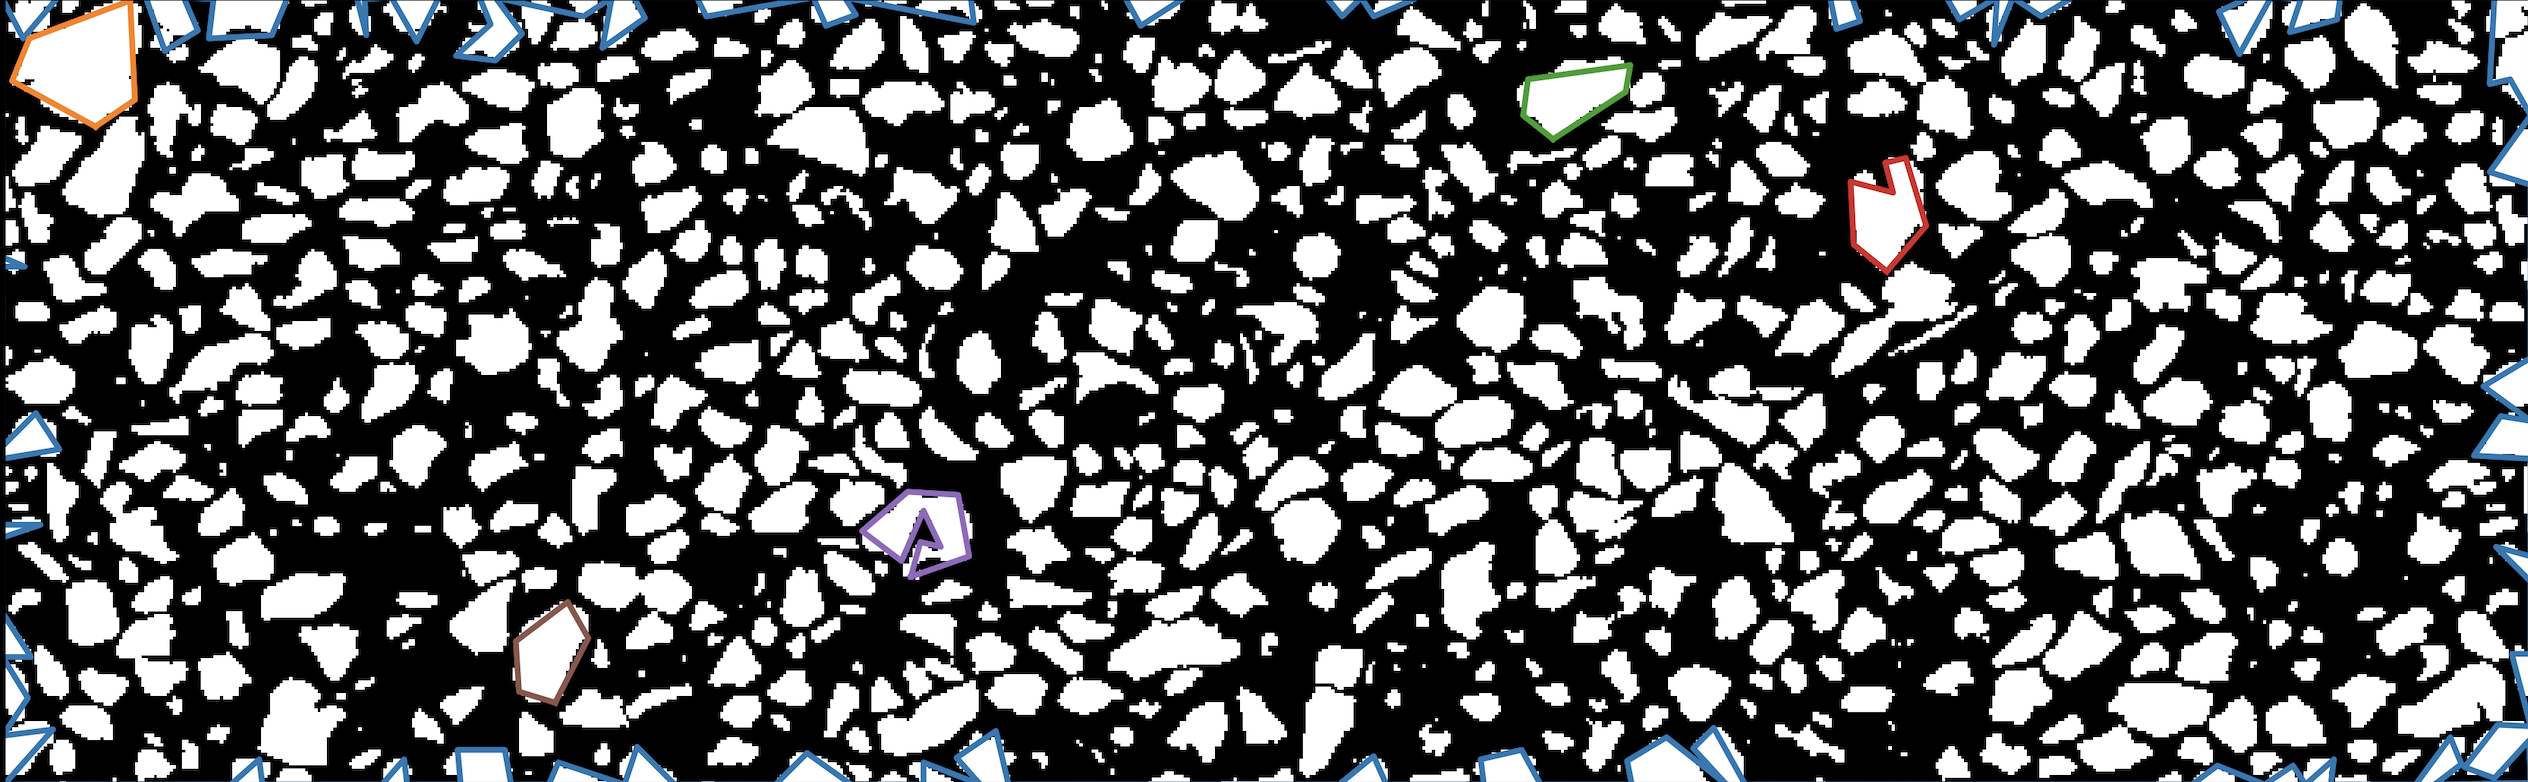
\includegraphics[width=0.7\textwidth]{size_500_5_5.png}
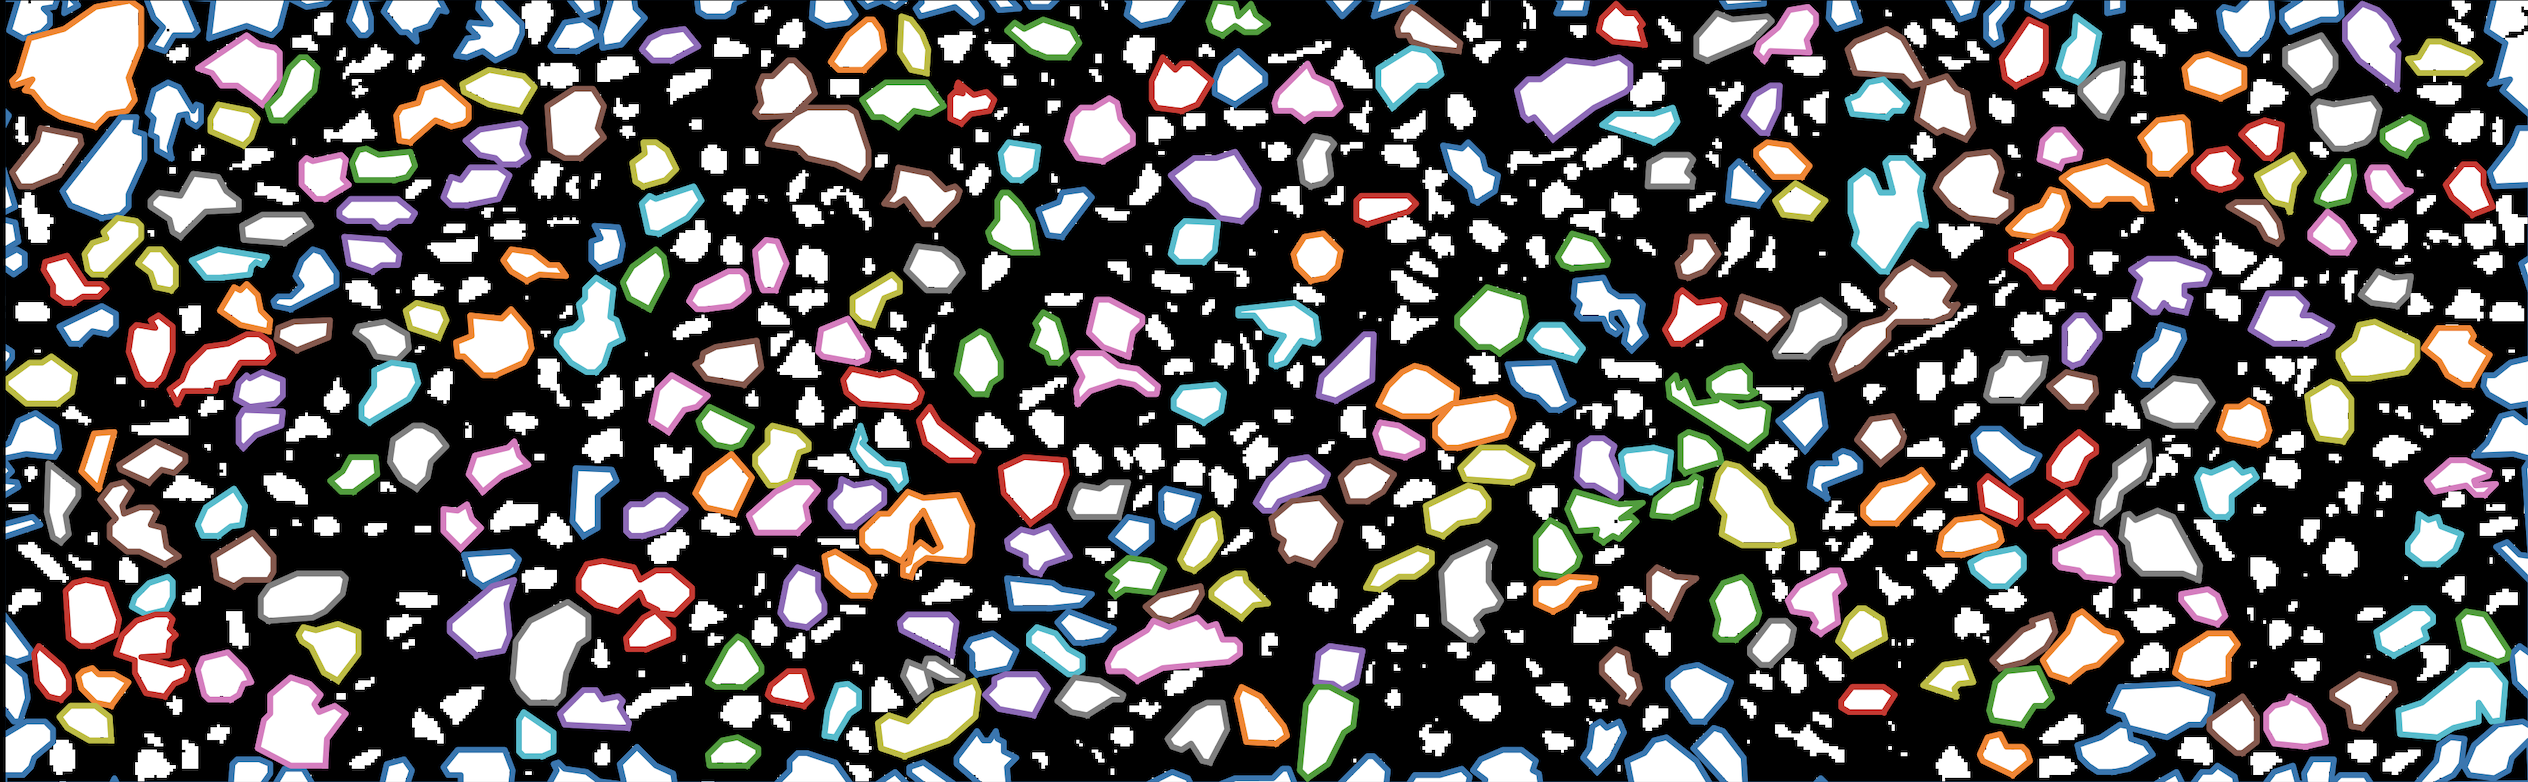
\includegraphics[width=0.7\textwidth]{size_100_1_1.png}
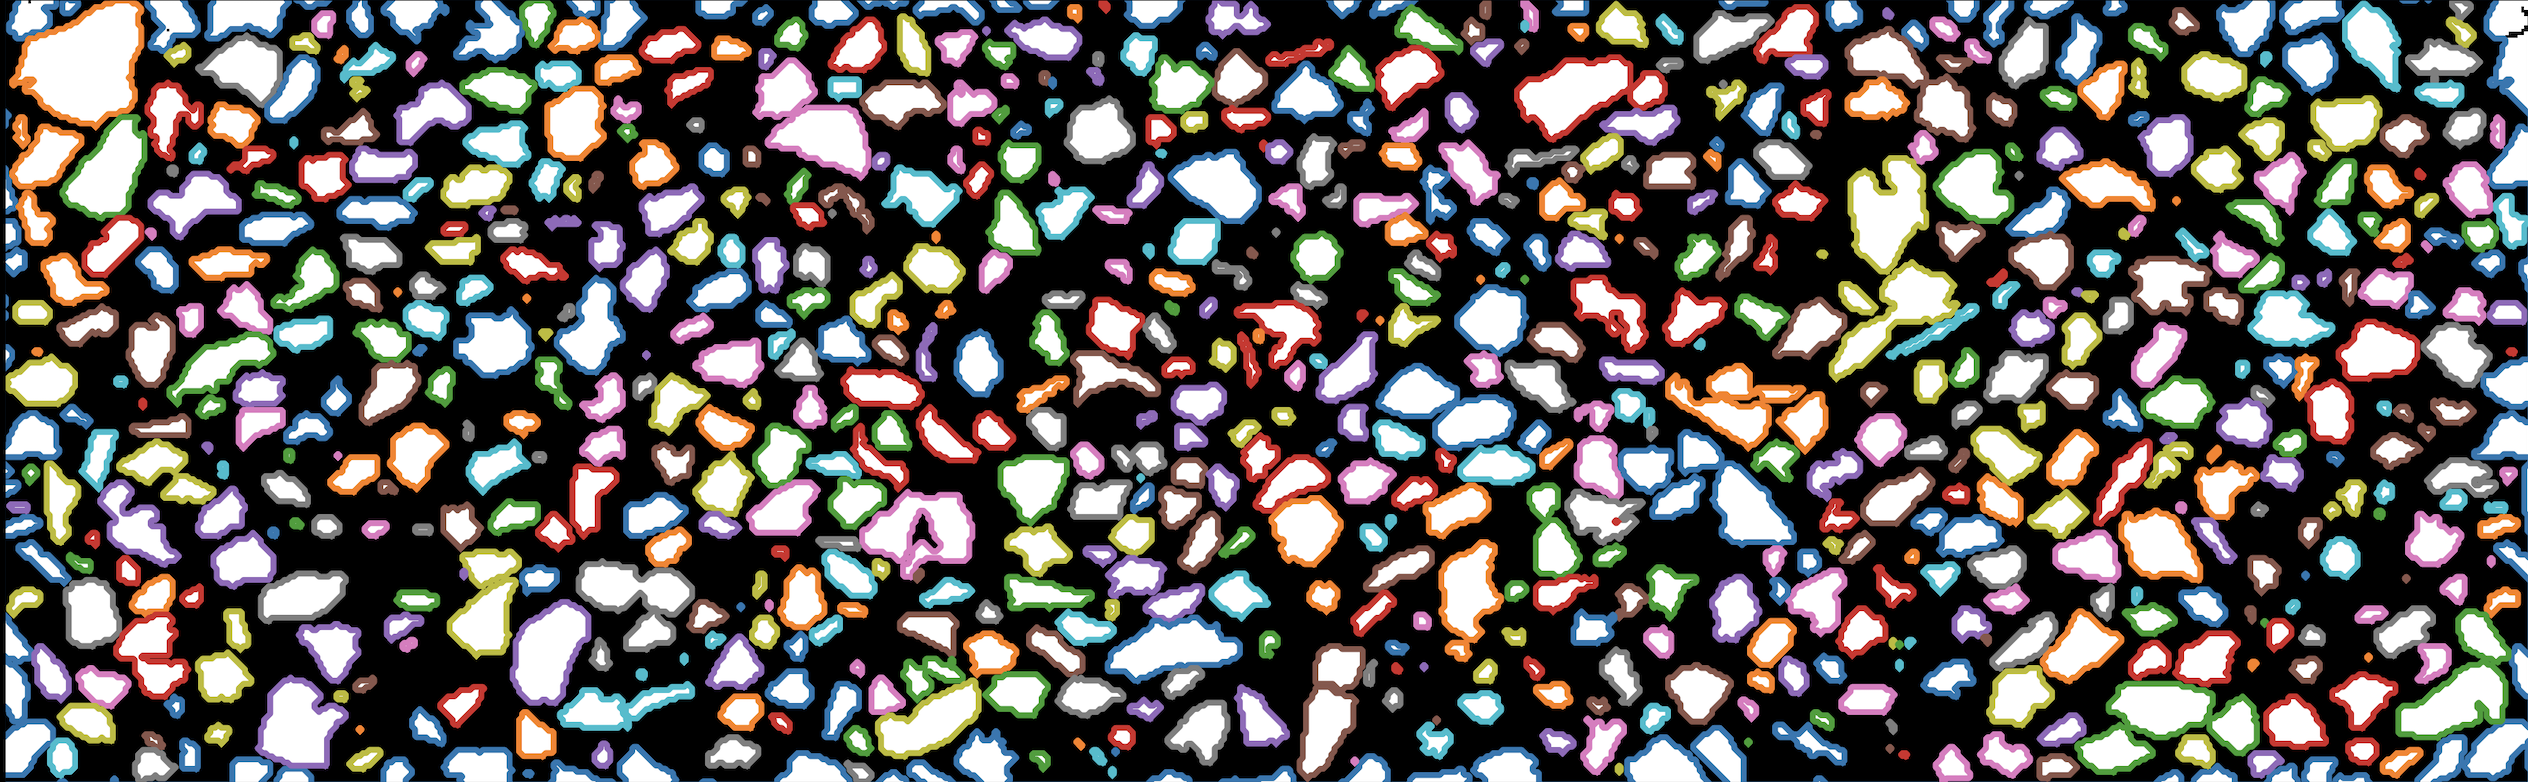
\includegraphics[width=0.7\textwidth]{size_0_0_0.png}
\caption{Extracted contours for minimum size of the cluster grains and tolerances for the polygon approximation of (top) 500, 5, 5, (middle) 100, 1, 1, and (bottom) 0, 0, 0, respectively.}
\label{sizes} 
\end{figure}

\subsection{Figure- and device- related parameters}
The figure parameter controls the line width of the contours on the output images, while the device parameter controls the width of the channels in the device microsystem (see the following subsection for details about the implemented device).

\subsection{Mesh-related parameters}
Currently the only input parameter for the mesh is the mesh size. Figure \ref{mesh} shows the generated mesh for two different mesh sizes.
\begin{figure}[h!]
\centering
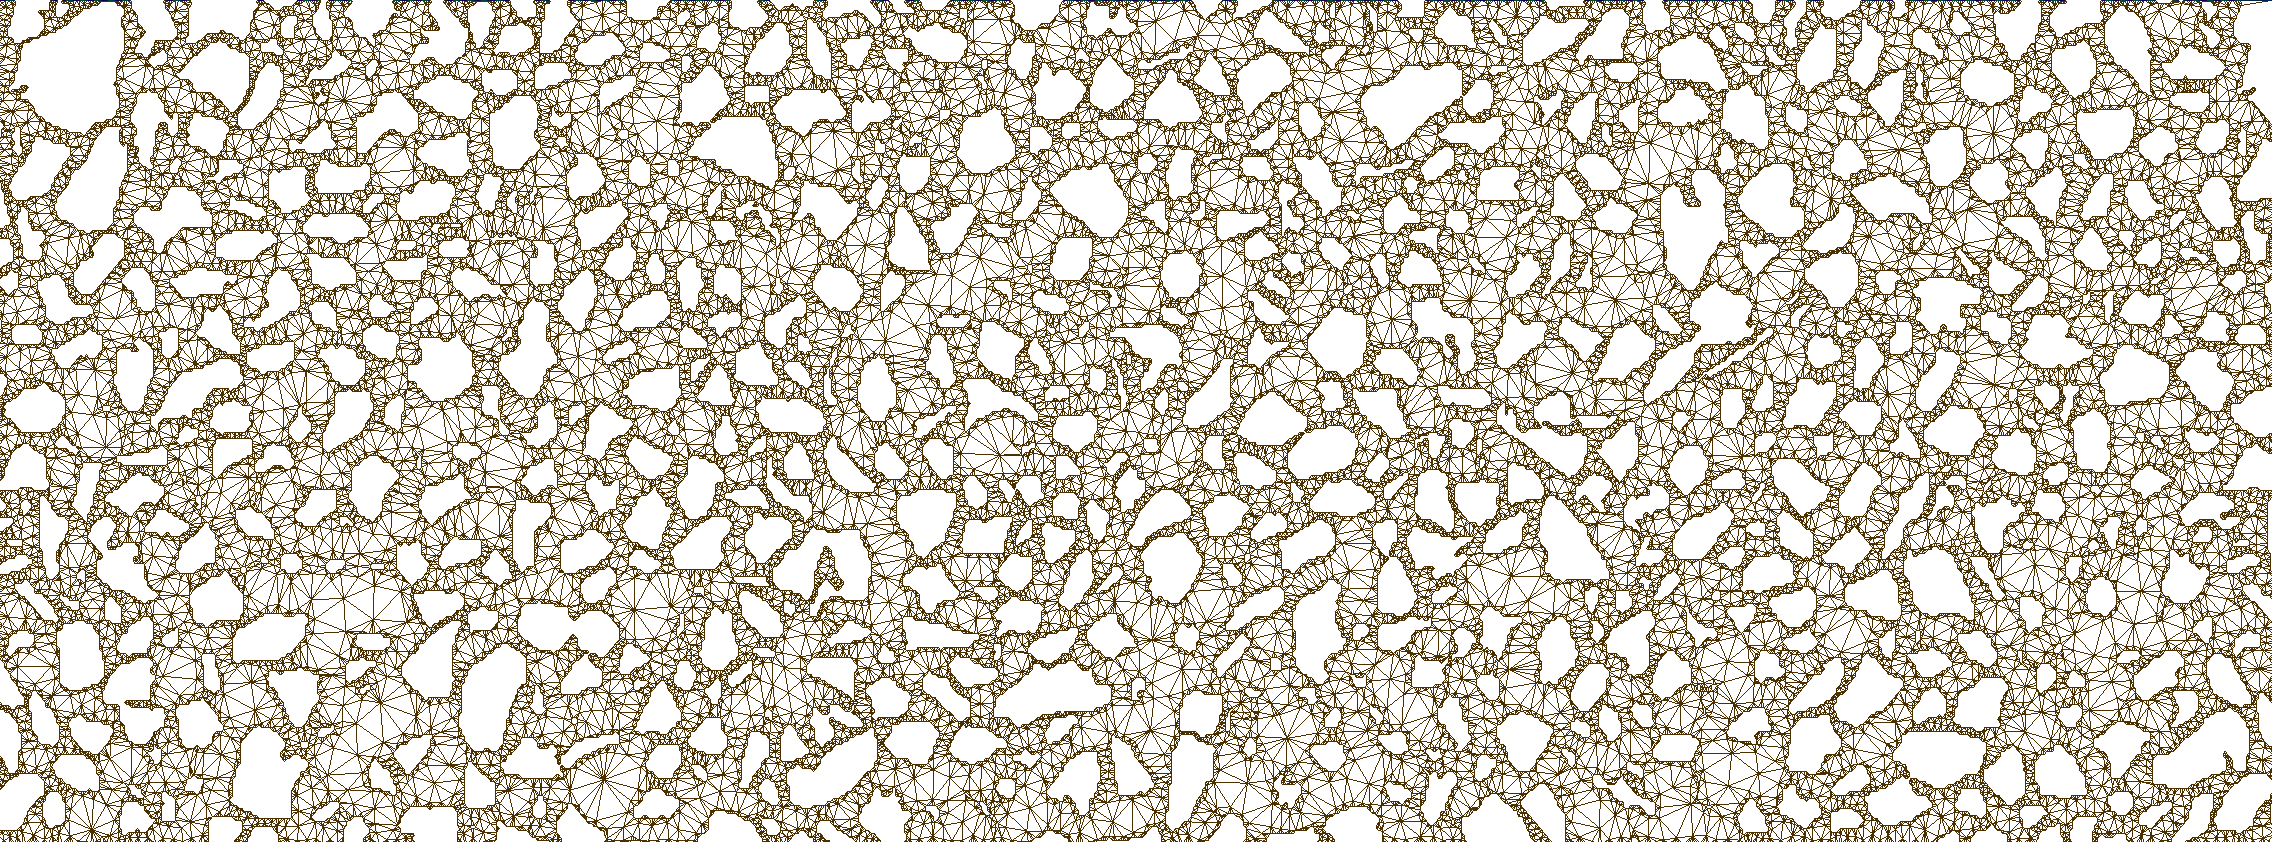
\includegraphics[width=0.7\textwidth]{mesh_1e4.png}
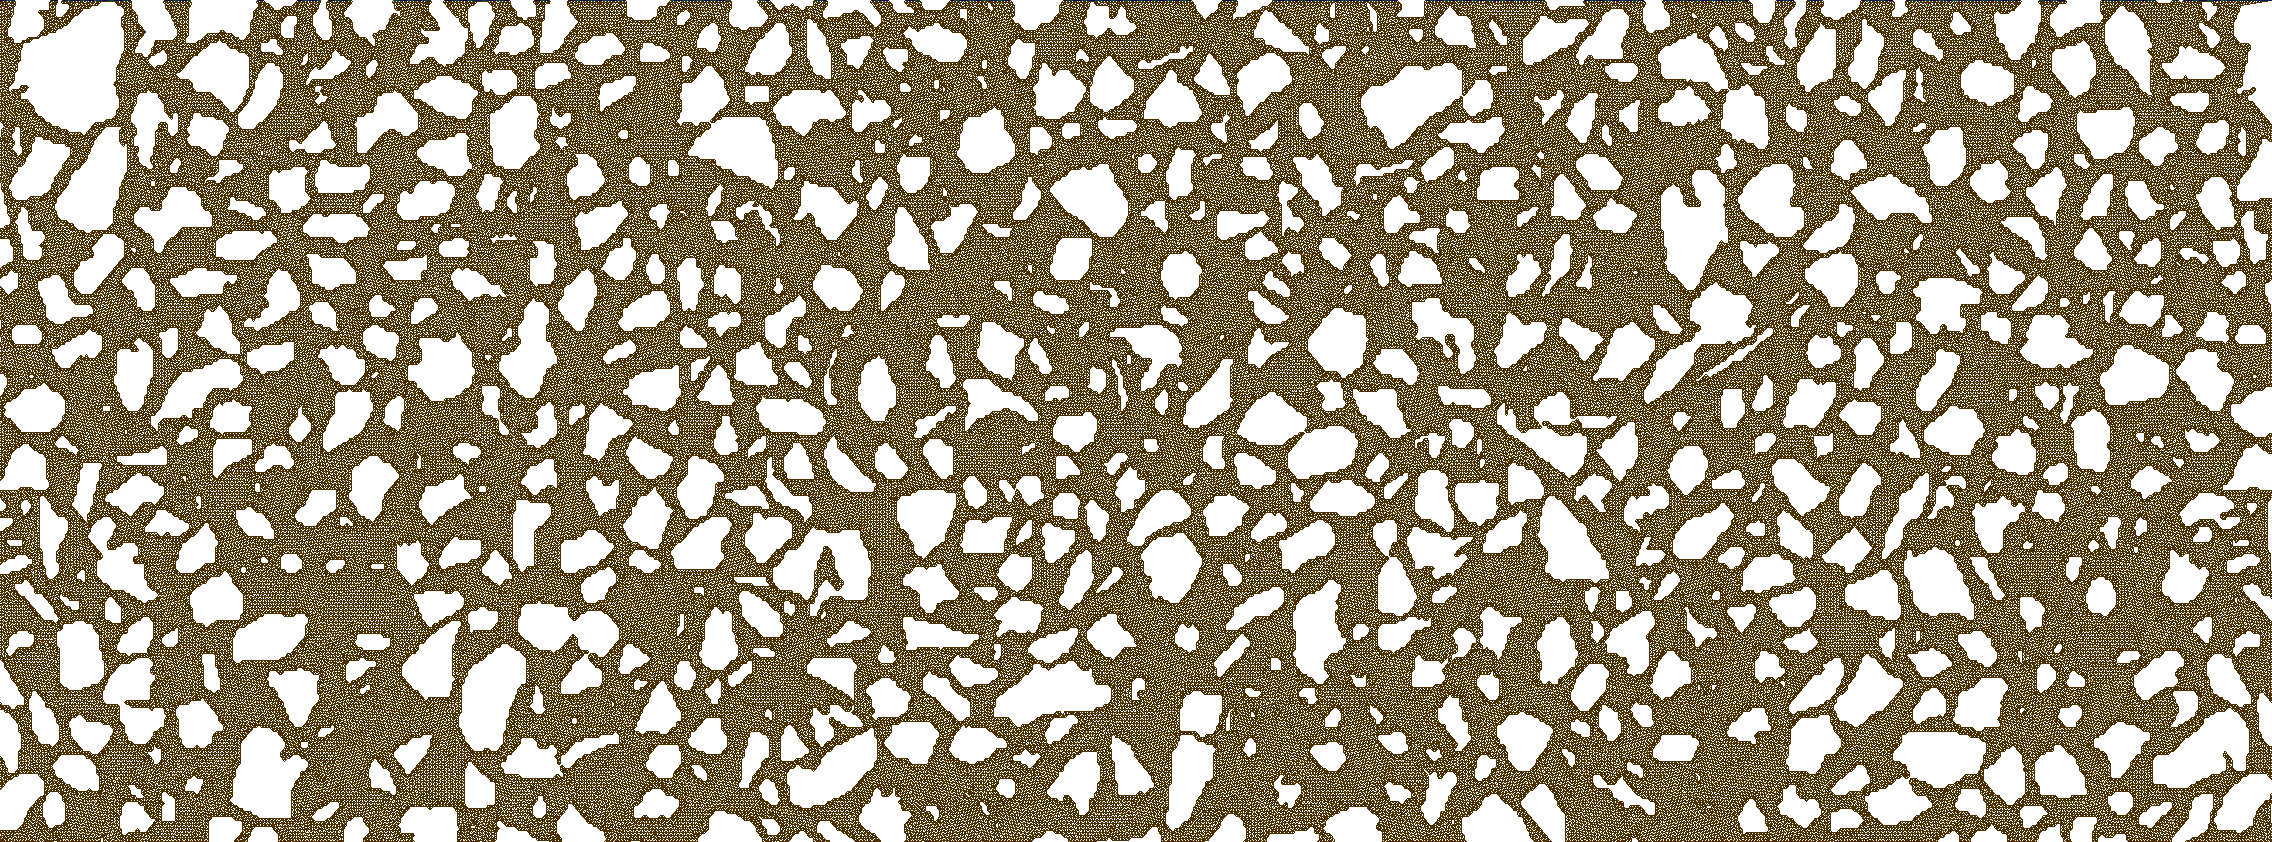
\includegraphics[width=0.7\textwidth]{mesh_1e5.png}
\caption{Two different generated meshes of sizes (top) 1e-4 and (bottom) 1e-5.}
\label{mesh} 
\end{figure}

There are currently two template files that define the configuration of the microsystem: image.mako and device.mako. The template image.mako considers that the flow is from top to bottom of the image, while device.mako creates the micromodel geometry as in \cite{Benali2019,Liu2022}. Then one could look at those files to modify the values (e.g., the flow direction or create quad elements for the mesh) or to define new micromodel geometries (e.g., a micromodel with a vertical cross-type shape). Figure \ref{modes} shows the geometry of the device micromodel.
\begin{figure}[h!]
\centering
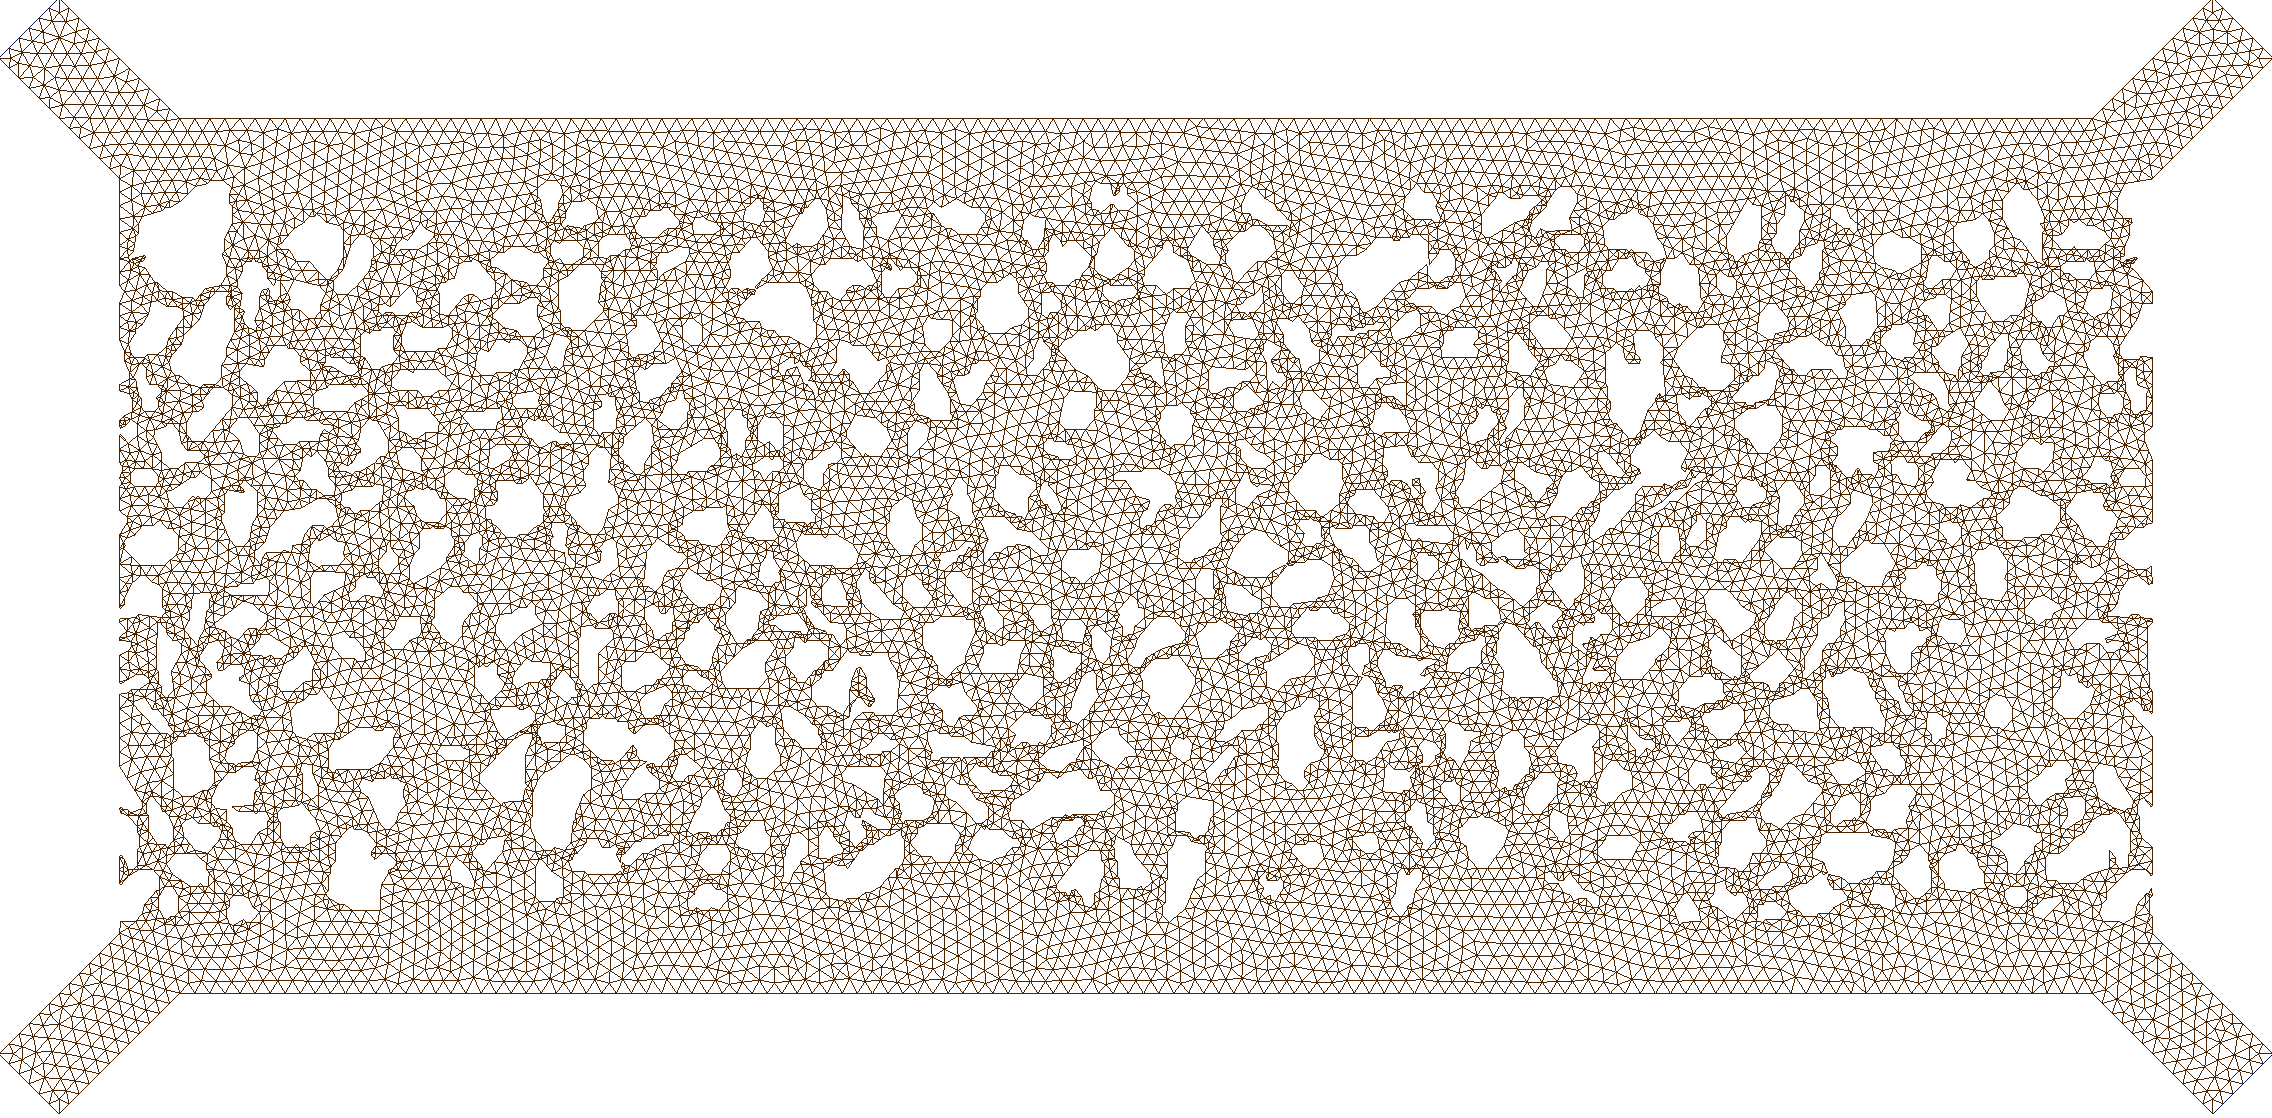
\includegraphics[width=0.7\textwidth]{device.png}
\caption{Geometry of the device mode.}
\label{modes} 
\end{figure}

\subsection{Remaining parameters}
The remaining parameters are OpenFOAM related. Refer to the online OpenFOAM resources for details about the simulator and \href{https://www.slideshare.net/ElwardiFadli/permeability-of-soils}{this nice presentation} using the OpenFOAM solver simpleFoam in another micromodel application. Details about the solver simpleFoam and mathematical model can be found \href{https://openfoamwiki.net/index.php/OpenFOAM_guide/The_SIMPLE_algorithm_in_OpenFOAM}{here}. Details about the solver scalarTransportFoam and mathematical model can be found \href{https://openfoamwiki.net/index.php/ScalarTransportFoam}{here}. 

\section{Generated files}
Figure \ref{output} shows the generated files in the selected output folder.
\begin{figure}[h!]
\centering
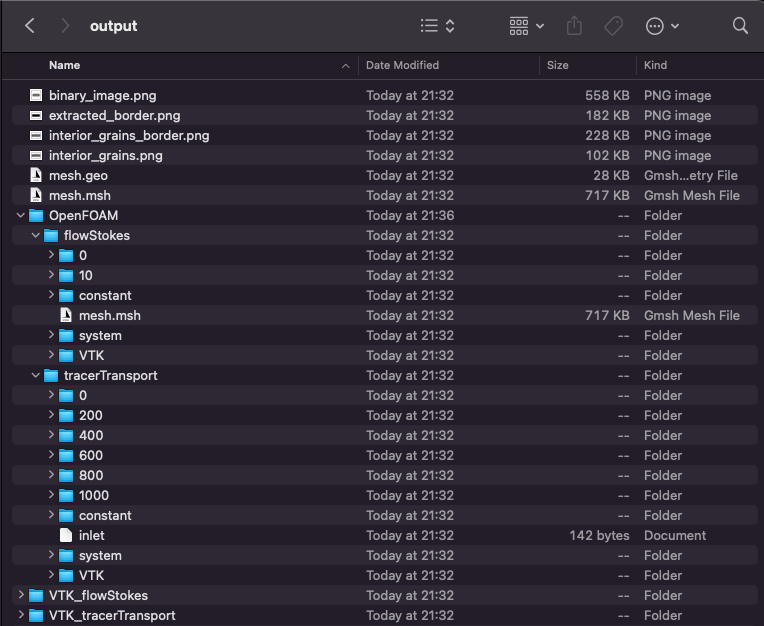
\includegraphics[width=0.7\textwidth]{output.png}
\caption{Generated files after executing pymm.}
\label{output} 
\end{figure}

Then after running pymm, one could modify the generated OpenFOAM related files and run directly the simulations calling the OpenFOAM solvers, e.g., to change additional tolerances that are not currently included in the parameters.txt file and/or to change the numerical schemes (see the OpenFOAM documentation \href{https://www.openfoam.com/documentation/user-guide/6-solving/6.2-numerical-schemes}{here}). Fig. \ref{simulations} show an example of simulation results.

\begin{figure}[h!]
\centering
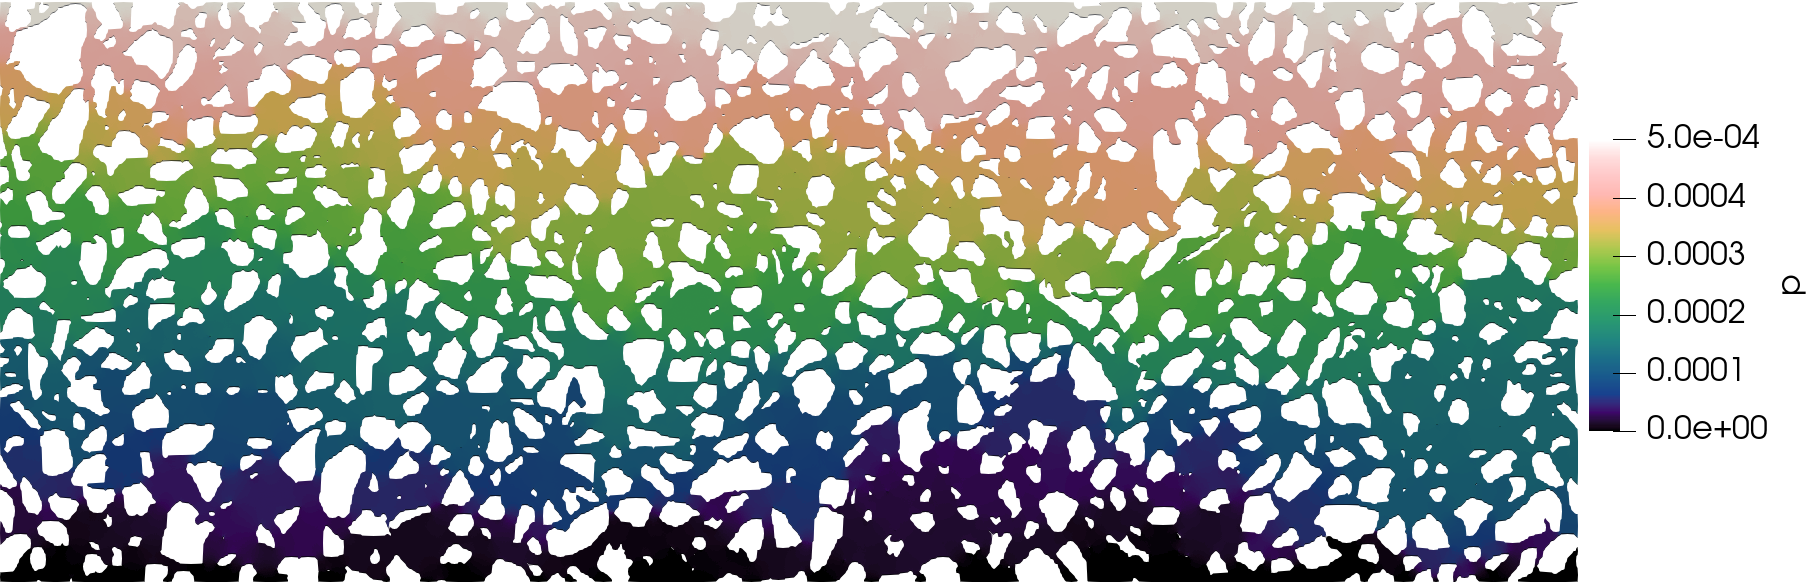
\includegraphics[width=0.7\textwidth]{pressure}
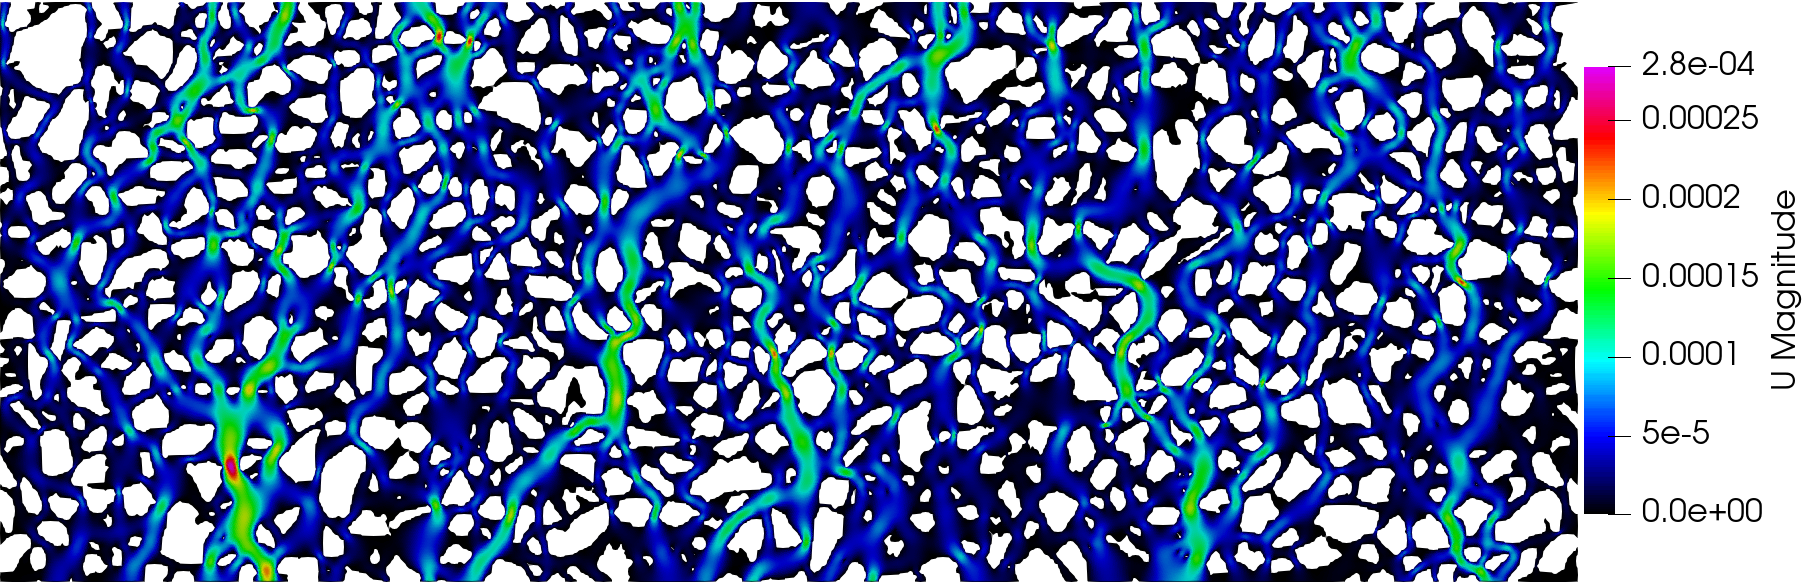
\includegraphics[width=0.7\textwidth]{velocity}
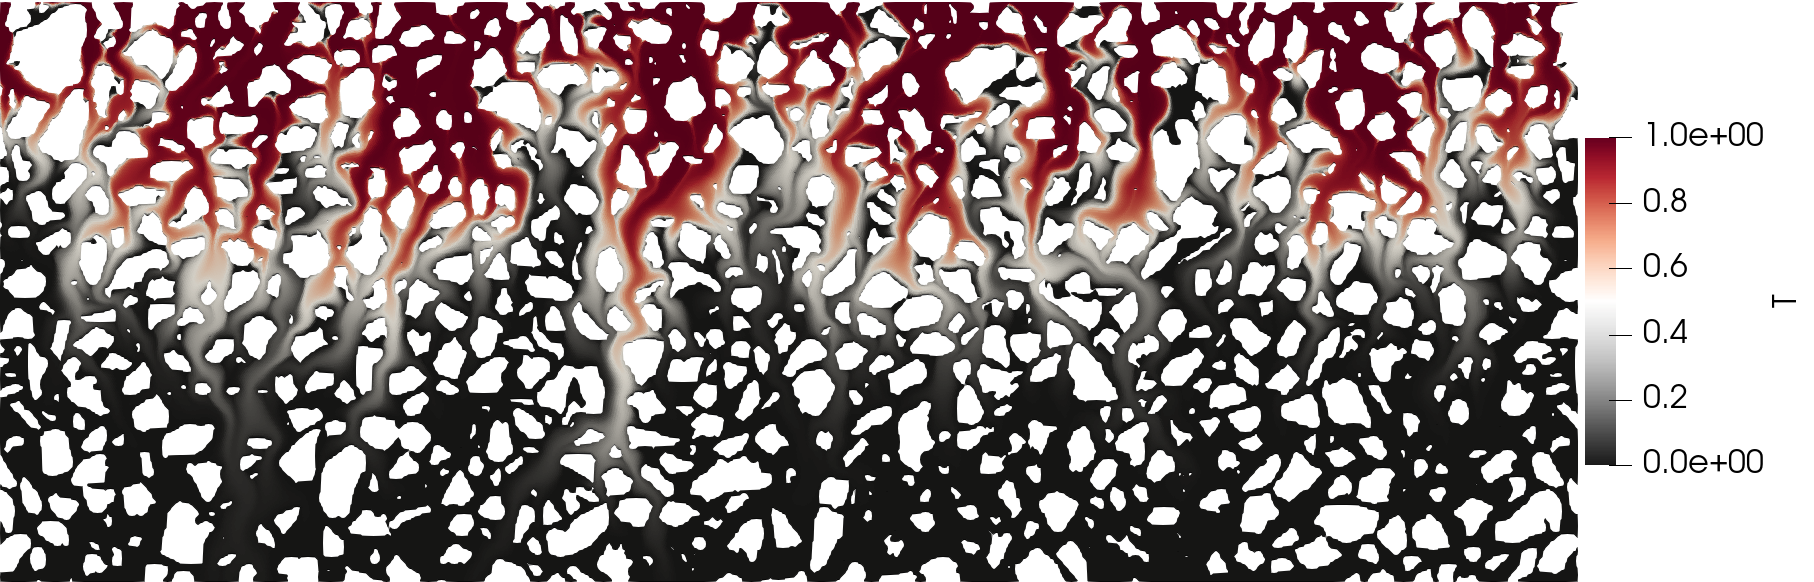
\includegraphics[width=0.7\textwidth]{tracer}
\caption{Simulation results of the (top) pressure, (middle) velocity, and (bottom) tracer concentration.}
\label{simulations} 
\end{figure}

\begin{thebibliography}{}

\bibitem[\protect\citeauthoryear{Benali}{2019}]{Benali2019}
Benali, B., 
Quantitative pore-scale analysis of CO$_2$ foam for CCUS.
Master thesis,
2019.
\href{https://hdl.handle.net/1956/21300}{https://hdl.handle.net/1956/21300}.

\bibitem[\protect\citeauthoryear{Liu et al.}{2022}]{Liu2022}
Liu, N., Haugen, M., Benali, B., Landa-Marbán, D., Fernø, M.A., 
Pore-scale spatiotemporal dynamics of microbial-induced calcium carbonate growth and distribution in porous media.
Submitted.

\bibitem[\protect\citeauthoryear{Gostick et al.}{2019}]{Gostick2019}
Gostick, J.T., Khan, Z.A., Tranter, T.G., Kok, M.D., Agnaou, M., Sadeghi, M., Jervis, R., 
PoreSpy: A python toolkit for quantitative analysis of porous media images.
Journal of Open Source Software 2019, 4, (37), 1296.

\bibitem[\protect\citeauthoryear{Van der Walt et al.}{2014}]{Walt2014}
Van der Walt, S., Schönberger, J.L., Nunez-Iglesias, J., Boulogne, F., Warner, J.D., Yager, N., Gouillart, E., Yu, T., 
scikit-image: image processing in Python. 
PeerJ 2014, 2, e453.

\bibitem[\protect\citeauthoryear{Geuzaine and Remacle}{2009}]{Geuzaine2009}
Geuzaine, C., Remacle, J. F., 
Gmsh: A 3‐D finite element mesh generator with built‐in pre‐and post‐processing facilities.
International journal for numerical methods in engineering 2009, 79, (11), 1309-1331.

\end{thebibliography}
\end{document}